\subsection{nicht schaltbar \hfill ME}
    \begin{footnotesize}
        \begin{center}
            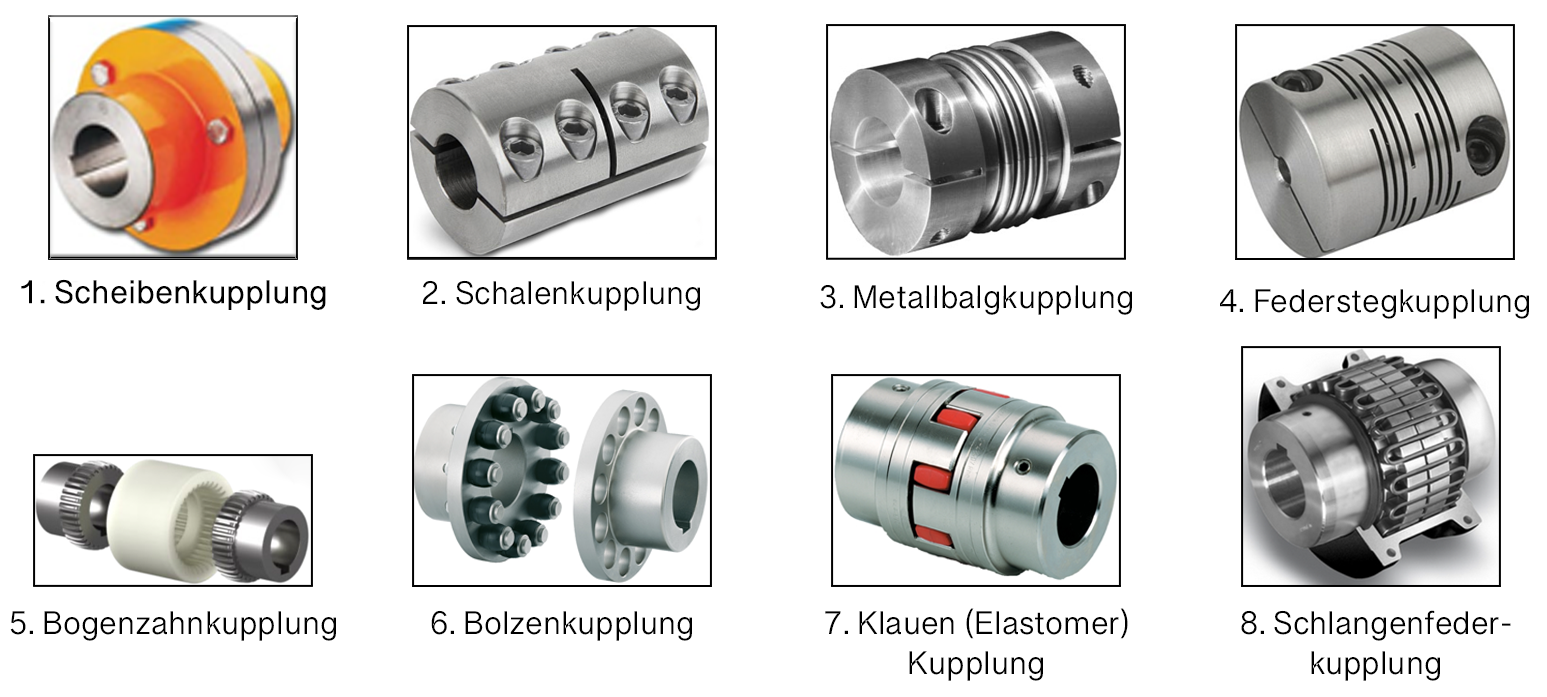
\includegraphics[width = 1.0\linewidth]{src/images/MAEIP_Kupplungen_nichtschaltbar}
                \begin{scriptsize}
                    \begin{tabular}{|c|c|c|c|c|c|c|c|}
                    \hline
                    \multirow{2}{0.01cm}{\null}& \multicolumn{2}{p{1.2cm}|}{\centering Drehnachgieb.} & \multicolumn{2}{p{0.9cm}|}{\centering Drehleist.} & \multicolumn{3}{p{0.9cm}|}{\centering Versatz} \bigstrut \\
                    \cline{2-8} & \multicolumn{1}{c|}{steif} & \multicolumn{1}{c|}{elastisch} & \multicolumn{1}{c|}{Moment} & \multicolumn{1}{c|}{Zahl} & \multicolumn{1}{c|}{Ax.} & \multicolumn{1}{c|}{Rad.} & \multicolumn{1}{c|}{Wink.} \bigstrut \\ \hline
                    1. & X & - & $\uparrow \uparrow / \uparrow\uparrow\uparrow$ & $\downarrow / \to$& none & none & none \bigstrut \\
                    \hline
                    2. & X & - & $\downarrow / \uparrow$ & $\downarrow / \to$ & none & none & none\bigstrut \\
                    \hline
                    3. & X & - & $\to / \uparrow$ & $\to / \uparrow$ & gut & gut & s. gut\bigstrut \\
                    \hline
                    4. & X & - & $\downarrow / \to$ & $\to / \uparrow$ & s. beg. & gut & gut\bigstrut \\
                    \hline
                    5. & X & - & $\uparrow / \uparrow\uparrow$ & $\to / \uparrow$ & gut & s. gut & gut\bigstrut \\
                    \hline
                    6. & - & X & $\uparrow / \uparrow\uparrow$ & $\downarrow / \to$ & gut & s. beg. & gut\bigstrut \\
                    \hline
                    7. & - & X & $\downarrow / \to$ & $\to / \uparrow$ & gut & s. beg. & gut\bigstrut \\
                    \hline
                    8. & - & X & $\to / \uparrow$ & $\downarrow / \to$ & gut & gut & gut\bigstrut \\
                    \hline
                    \end{tabular}
                \end{scriptsize}
        \end{center}
    \end{footnotesize}

    \subsubsection{Kupplungen mit grossem Radialversatz \hfill ME}
        \begin{footnotesize}
            \begin{center}
                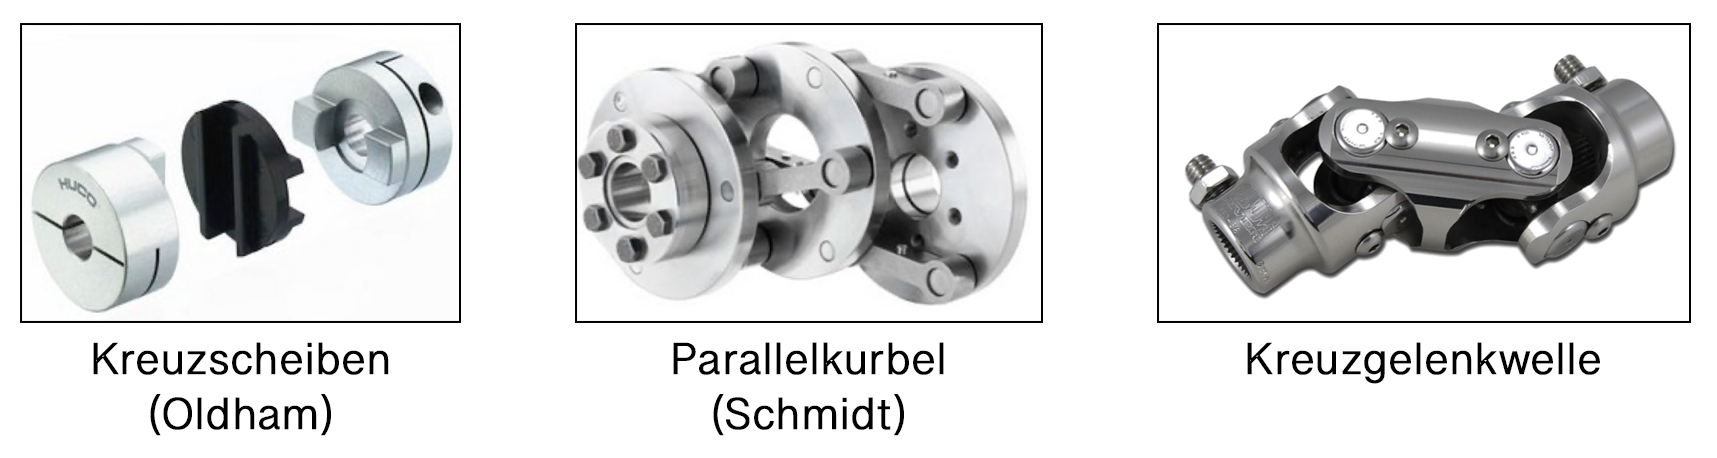
\includegraphics[width = 0.8\linewidth]{src/images/MAEIP_KupplungenRadialversatz}
            \end{center}
        \end{footnotesize}
